\subsubsection{26.01.2016}
\textit{\textbf{Time frame:}} 17:00-21:00

The moving mounts for ribs on the elevator were recreated (figure \ref{Elevator3.6}, \ref{Elevator3.7}). There were applied white collars, which were sliding along the 10 cm axes. This construction had less friction and was more reliable. These details were not finished during the current meeting.

\begin{figure}[H]
	\begin{minipage}[h]{0.47\linewidth}
		\center{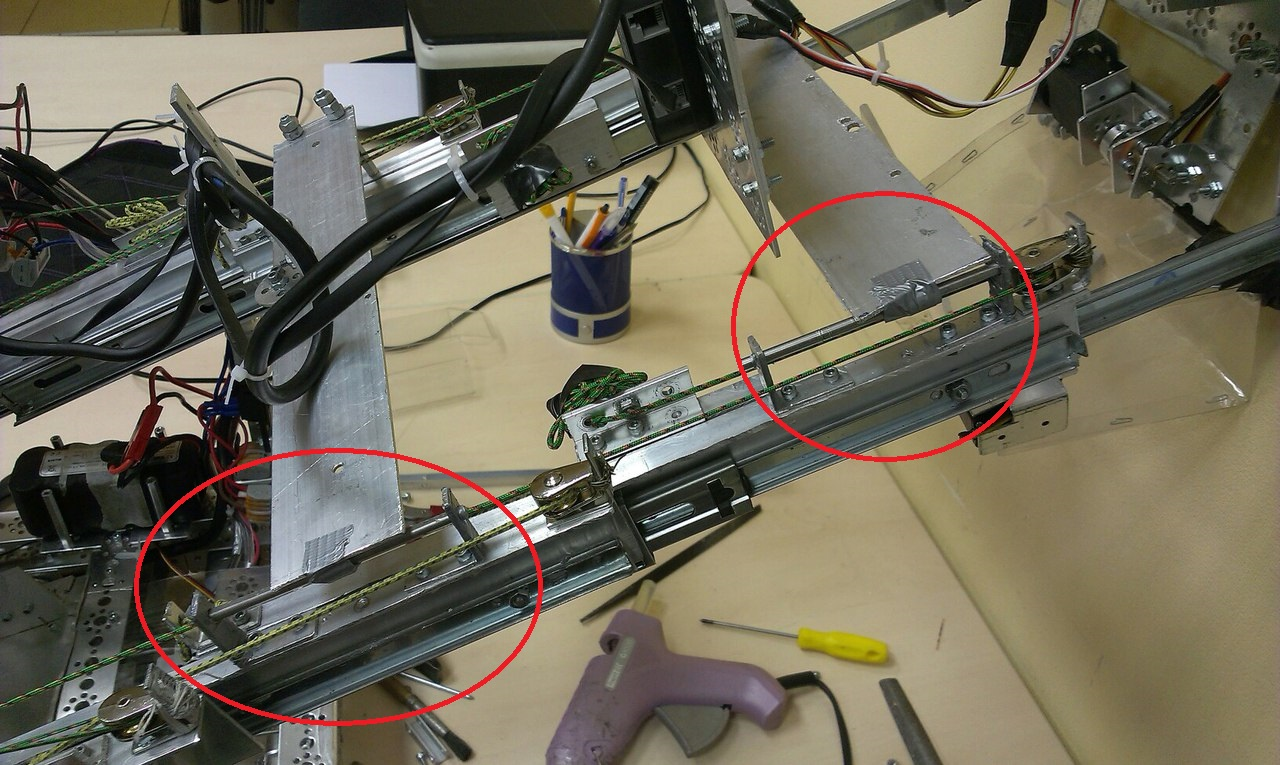
\includegraphics[scale=0.2]{3Engineering/5Team_meetings/days_of_meetings/2016.01.26/images/01}}
		\caption{Convenient movable mounts of the ribs}
		\label{Elevator3.6}
	\end{minipage}
	\hfill
	\begin{minipage}[h]{0.47\linewidth}
		\center{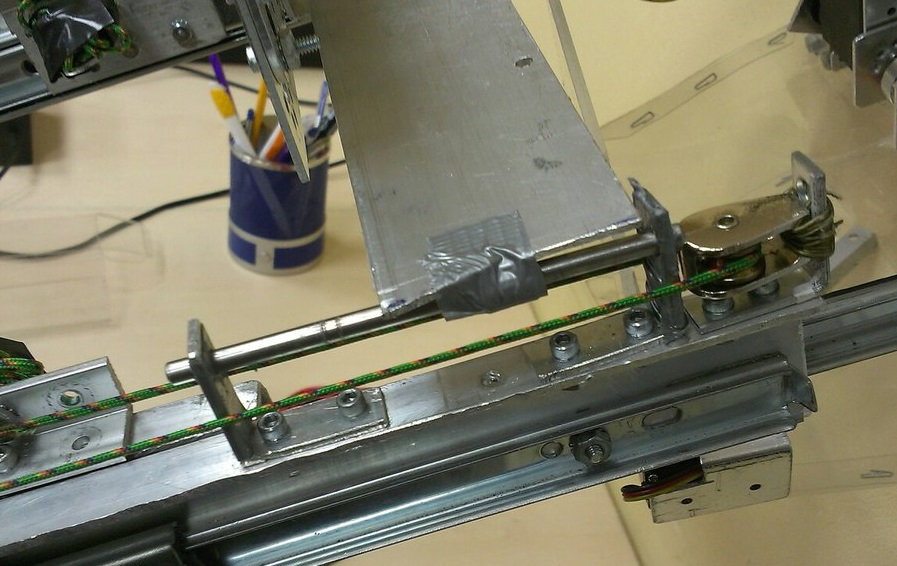
\includegraphics[scale=0.25]{3Engineering/5Team_meetings/days_of_meetings/2016.01.26/images/02}}
		\caption{The mount of the rib}
		\label{Elevator3.7}
	\end{minipage}
\end{figure}

After a number of tests, the brushes on the gripper were set in the most effective position.

It was created a protection from debris at the back of the robot (figure \ref{Protection1.1}).

The protection of the area under the bucket from debris was recreated with a layer of PET (figure \ref{Protection1.2}).

\begin{figure}[H]
	\begin{minipage}[h]{0.47\linewidth}
		\center{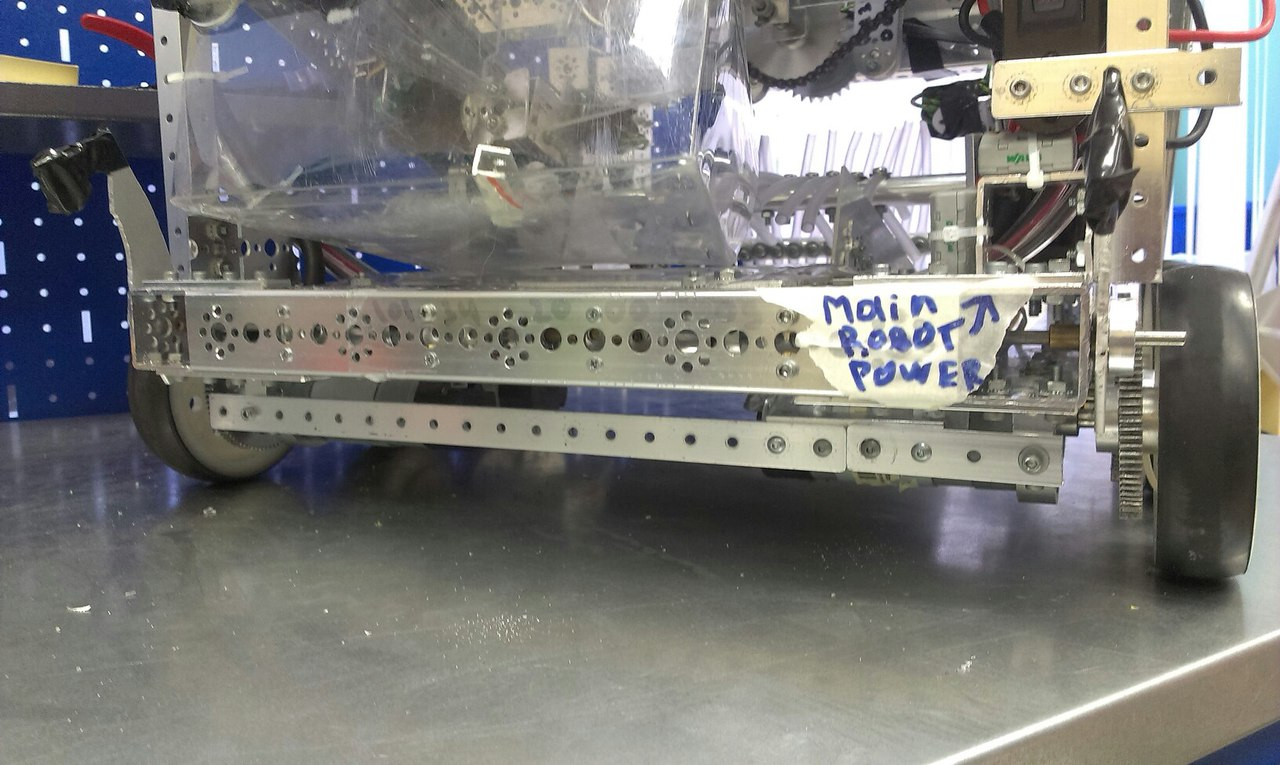
\includegraphics[scale=0.2]{3Engineering/5Team_meetings/days_of_meetings/2016.01.26/images/03}}
		\caption{Protection from debris 1}
		\label{Protection1.1}
	\end{minipage}
	\hfill
	\begin{minipage}[h]{0.47\linewidth}
		\center{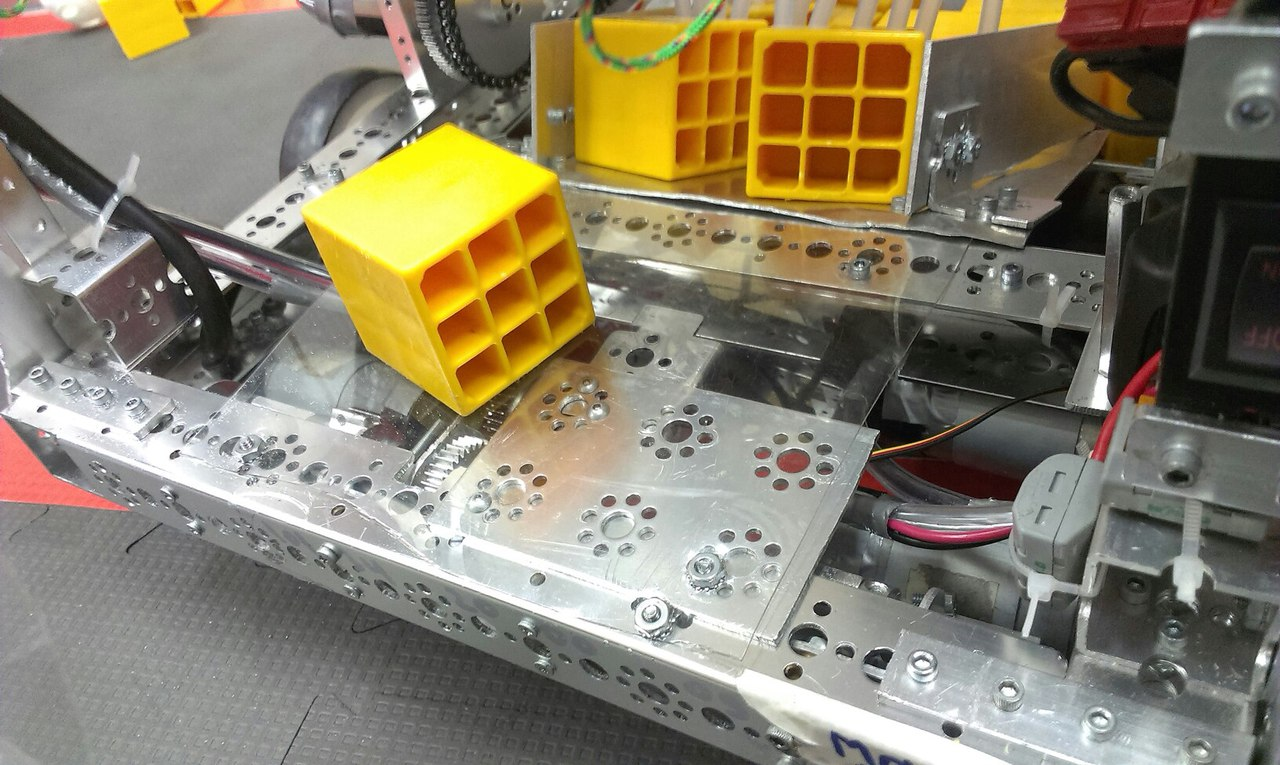
\includegraphics[scale=0.22]{3Engineering/5Team_meetings/days_of_meetings/2016.01.26/images/04}}
		\caption{Protection from debris 2}
		\label{Protection1.2}
	\end{minipage}
\end{figure}
